\section{Sistemas operativos}

\subsection{Android}

Android es un sistema operativo móvil creado por \textbf{Google} y cimentado sobre el kernel de Linux y otros softwares de código libre. Está diseñado principalmente para dispositivos con pantallas táctiles como smartphones o tablets, aunque a día de hoy se encuentra ya extendido a todo tipo de dispositivos como en televisiones inteligentes con AndroidTV o en automóviles con AndroidAuto. Ha sido un sistema operativo de obligado uso en este desarrollo al ser \emph{All For One} un sistema dirigido a dispositivos que lo usan. Se utilizó a lo largo de todo el desarrollo para probar la aplicación móvil desarrollada en diversos entornos y versiones. 

Las versiones 8 y 9 fueron empleadas a través de los emuladores de \nameref{ssec:android_studio}, el hardware replicado con los mismos fue el del teléfono móvil Google Pixel 4. La versión 10 fue empleada en un teléfono real de la marca Xiaomi MiA2 tanto por medio de conexión con el \acrshort{ide} como por medio de la instalación de la \acrshort{apk}. Por último, la versión más actual en el momento de desarrollo, \textbf{Android 11}, fue utilizado en el terminal habitual del desarrollador, un Xiaomi Redmi Note 10 Pro de menos de un año de antigüedad. Como en el caso del smartphone anterior, fue ejecutado con la emulación de la aplicación con el \acrshort{ide} y por medio de la instalación de la \acrshort{apk}.

Para más información: \href{https://www.android.com/}{https://www.android.com/}

\subsection{Fedora Workstation}
\label{so:fedora_workstation}

Fedora Linux es una distribución Linux desarrollada por la comunidad bajo un proyecto del mismo nombre que el sistema operativo. Su principal patrocinador es la empresa \textbf{Red Hat}. Desde el lanzamiento de su versión 30, Fedora cuenta con cinco ediciones disponibles de su sistema operativo con énfasis en diferentes ámbitos: \textbf{Workstation}, para ordenadores personales; \textbf{Server}, para servidores; \textbf{CoreOS}, para la computación en la nube; \textbf{Silverblue}, para flujos de trabajo basados en contenedores; y \textbf{IoT}, para dispositivos del internet de las cosas.

\begin{figure}[H]
    \centering
    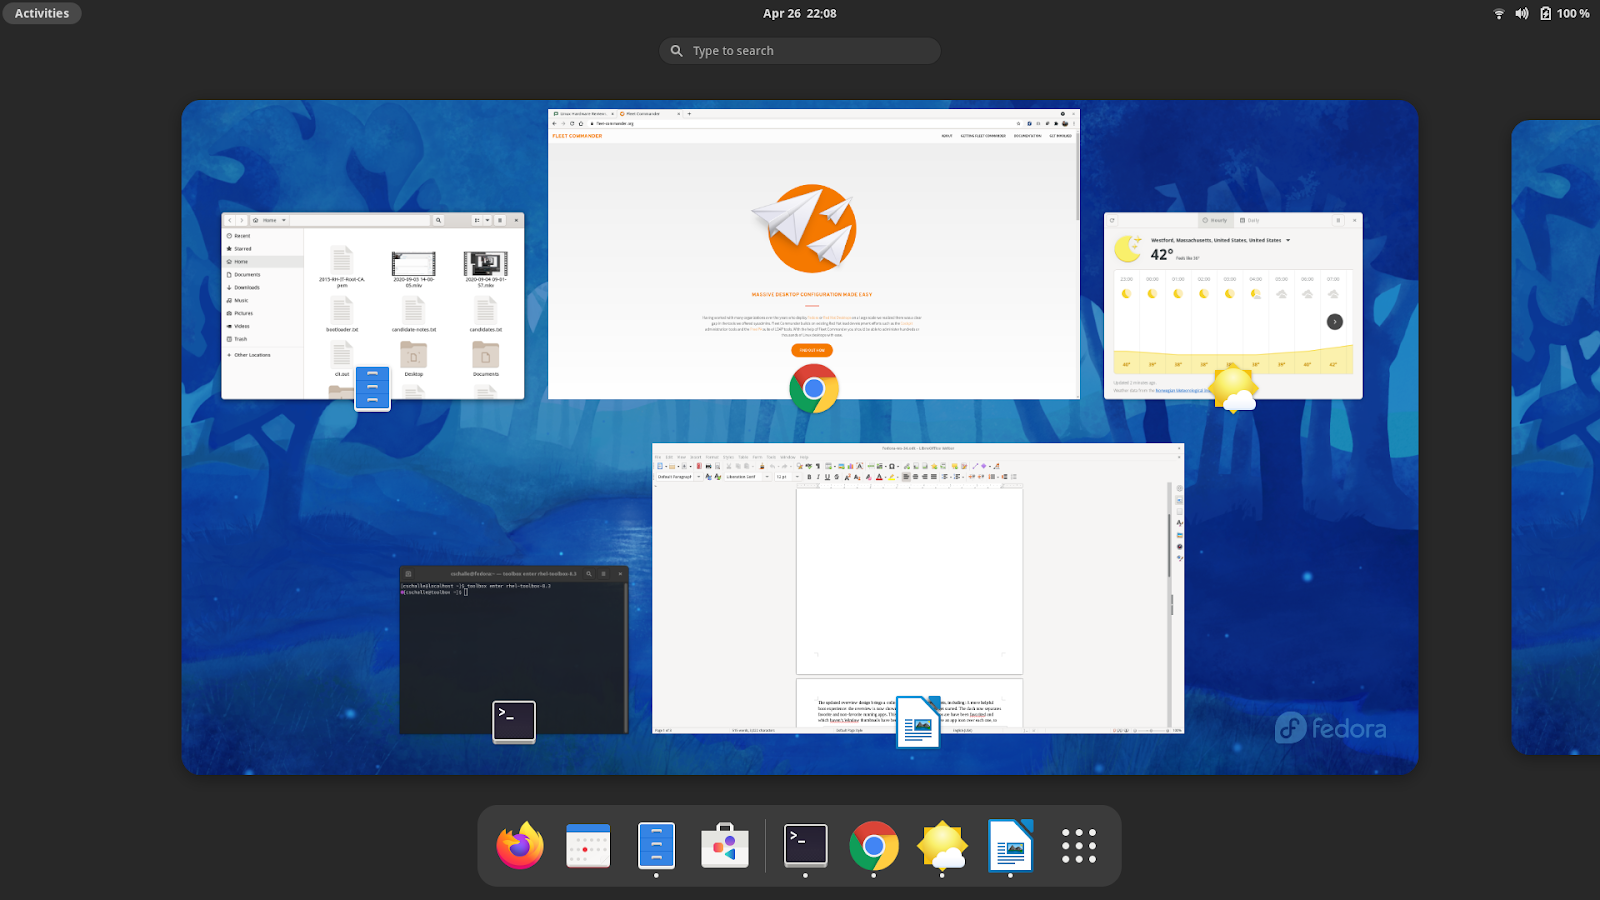
\includegraphics[width=0.75\textwidth]{Implementación/fedora-desktop.png}
    \caption{Escritorio de Fedora Workstation}
    \label{fig:fedora}
\end{figure}

\newpage
En este desarrollo se utilizó \textbf{Fedora Workstation 34} en un portátil Lenovo Ideapad 3 de última generación. Workstation utiliza GNOME 40 como escritorio y es un sistema operativo creado con el desarrollo de software en mente, lo que lo convirtió en una gran herramienta para la etapa de implementación, facilitando y agilizando el desarrollo. Fue el sistema operativo principal de desarrollo.

Para más información: \href{https://getfedora.org/en/workstation/}{https://getfedora.org/en/workstation/}

\subsection{Windows}

El último sistema operativo utilizado a lo largo del proceso de implementación por parte del equipo de desarrollo fue \textbf{Windows 10}, el sistema operativo lanzado por \textbf{Microsoft} en el año 2015. Fue lanzado de forma gratuita para los usuarios de sus versiones anteriores\footnote{Windows 7, 8 y 8.1} por medio de actualizaciones y de la Windows Store. Actualmente se encuentra dentro de los diez años de soporte garantizados para cualquier sistema operativo de la familia Windows. En marzo de 2020 alcanzó el millardo de usuarios\cite{warren2020}, dos años después de superar a Windows 7 en usuarios. A día de hoy ya ha sida lanzado una versión más reciente, \textbf{Windows 11}.

Esta plataforma de software se utilizó sobre un PC de configuración personal cuando por motivos de desplazamiento no se podía utilizar el entorno habitual. Para más información: \href{https://www.microsoft.com/es-es/windows/windows-10-specifications}{https://www.microsoft.com/es-es/windows/windows-10-specifications}

\subsubsection{WSL2}

De cara a ofrecer la mayor consistencia posible en los entornos de desarrollo, durante la creación del sistema con el sistema operativo Windows se hizo uso de la herramienta \textbf{Windows Subsystem for Linux} con una imagen de \textbf{Ubuntu 20.04 LTS}. Esta herramienta proporciona una capa de compatibilidad con sistemas operativos Linux ejecutada nativamente sobre Windows. De esta forma el desarrollo se pudo llevar a cabo sobre una base UNIX en las dos plataformas y sistemas operativos empleados durante la creación del sistema.

Para más información: \href{https://docs.microsoft.com/en-us/windows/wsl/about}{https://docs.microsoft.com/en-us/windows/wsl/about}